\documentclass[11pt,oneside,onecolumn,openany,spanish]{book}

\usepackage{lmodern}
\usepackage[T1]{fontenc}
\usepackage{babel}
%\usepackage[spanish,activeacute]{babel}
\usepackage{mathtools}
\usepackage{multirow} 
\usepackage{tikz}
\usetikzlibrary{automata,positioning}
\usetikzlibrary{babel}

\title{Pr�ctica PL}
\author{Elena Kaloyanova Popova y �lvaro Borja Velasco Garc�a}
\date{2018}

\begin{document}
% cuerpo del documento
\newcommand{\mystar}{{\fontfamily{lmr}\selectfont$\star$}}
\newcommand\tab[1][0.7cm]{\hspace*{#1}}

\maketitle
\tableofcontents % crea el �ndice

%---------------------------------------------------------------------
%                   Cap�tulo 1 - Analizador l�xico
%---------------------------------------------------------------------
\chapter{Fase 1: Analizador l�xico}

%---------------------------------------------------------------------
\section{Clases L�xicas}
%---------------------------------------------------------------------
\label{cap1:sec:clases_lexicas}
Todo programa consta de dos secciones: una para las declaraciones y otra para las instrucciones, separadas por un token "`\&\&"'. La secci�n de declaraciones est� formada por una serie de declaraciones compuestas por el nombre de tipo y el de variable y separadas por un punto y coma. La secci�n de instrucciones, por su parte, consta de una serie de asignaciones (variable=expresi�n), separadas tambi�n por un punto y coma.
Las clases l�xicas que hemos considerado para representar los tokens del lenguaje son las siguientes:

\begin{itemize}
	\item \textbf{SEC:} Representa el seccionador de las dos partes del programa ("`\&\&"').
	\item \textbf{NUM:} Palabra reservada "`num"'.
	\item \textbf{BOOL:} Palabra reservada "`bool"'.
	\item \textbf{VAR:} Representa el nombre de la variable. Comienza necesariamente por una letra, seguida por una secuencia de cero o m�s letras, d�gitos o el s�mbolo "`\_"'.
	\item \textbf{ASIG:} Representa el signo igual de las asignaciones.
	\item \textbf{NXT:} Representa el signo "`;"' que marca el comienzo de la siguiente instrucci�n.
	\item \textbf{TRUE:} Palabra reservada "`true"'.
	\item \textbf{FALSE:} Palabra reservada "`false"'.
	\item \textbf{NUMR:} Representa un n�mero real. Puede empezar opcionalmente con un signo seguido de una secuencia de uno o m�s digitos cualesquiera, pudiendo poner ceros no significativos a la izquierda. Puede opcionalmente estar seguido por una parte decimal y/o una parte exponencial.
	\item \textbf{MAS:} Operador suma (\textbackslash +).
	\item \textbf{MENOS:} Operador resta (\textbackslash -).
	\item \textbf{POR:} Operador multiplicaci�n (\textbackslash *).
	\item \textbf{DIV:} Operador divisi�n (/).
	\item \textbf{AND:} Palabra reservada "`and"'.
	\item \textbf{OR:} Palabra reservada "`or"'.
	\item \textbf{NOT:} Palabra reservada "`not"'.
	\item \textbf{MAY:} Operador mayor (>).
	\item \textbf{MEN:} Operador menor (<).
	\item \textbf{MAYI:} Operador mayor o igual (>=).
	\item \textbf{MENI:} Operador menor o igual (<=).
	\item \textbf{IGUAL:} Operador igual a (==).
	\item \textbf{DIST:} Operador distinto a (!=).
	\item \textbf{PAP:} Signo de apertura de par�ntesis.
	\item \textbf{PCI:} Signo de cierre de par�ntesis.
	\item \textbf{EOF:} Representa el final de fichero.

\end{itemize}
%---------------------------------------------------------------------
\section{Especificaci�n Formal}
%---------------------------------------------------------------------
\label{cap1:sec:especificacion_formal}

Las definiciones regulares correspondientes a las clases l�xicas definidas son:

	\textbf{(\mystar )  SEC:} [\&][\&]
	
	\textbf{(\mystar ) VAR:} \underline{LETRA}([\underline{LETRA}|\underline{DIG}|\textbackslash \_]*)
	
	\tab \textbf{LETRA:} ([a-z,A-Z])
	
	\tab \textbf{DIG:} ([0-9])
	
	\textbf{(\mystar ) NUM:} ([n][u][m])
	
	\textbf{(\mystar ) BOOL:} ([b][o][o][l])
	
	\textbf{(\mystar ) TRUE:} ([t][r][u][e])
	
	\textbf{(\mystar ) FALSE:} ([f][a][l][s][e])
	
	\textbf{(\mystar ) NUMR:} \underline{SIGNO}?(\underline{DIG}+(\underline{DEC})?(\underline{EX})?) 
	
	\tab \textbf{DEC:} (\textbackslash .)\underline{DIG}+ 
	
	\tab \textbf{EX:} [e|E](\underline{SIGNO}?\underline{DIG}+)
	
	\tab \textbf{SIGNO:} [\textbackslash +,\textbackslash -] 
	
	\tab \textbf{DIG:} [0-9]
	
	\textbf{(\mystar ) AND:} ([a][n][d])
	
	\textbf{(\mystar ) OR:} ([o][r])
	
	\textbf{(\mystar ) NOT:} ([n][o][t])
	
	\textbf{(\mystar ) MAS:} (\textbackslash +)
	
	\textbf{(\mystar ) MENOS:} (\textbackslash -)
	
	\textbf{(\mystar ) DIV:} (/)
	
	\textbf{(\mystar ) POR:} (\textbackslash *)
	
	\textbf{(\mystar ) MAY:} (>)
	
	\textbf{(\mystar ) MEN:} (<)
	
	\textbf{(\mystar ) MAYI:} ([>][=])
	
	\textbf{(\mystar ) MENI:} ([<][=])
	
	\textbf{(\mystar ) IGUAL:} ([=][=])
	
	\textbf{(\mystar ) DIST:} ([!][=])
	
	\textbf{(\mystar ) ASIG:} (=)
	
	\textbf{(\mystar ) NXT:} (;)
	
	\textbf{(\mystar ) PAP:} (\textbackslash $($)
	
	\textbf{(\mystar ) PCIERRE:} (\textbackslash $)$)
	
	\textbf{(\mystar ) SEP:} ["` "',\textbackslash t,\textbackslash n,\textbackslash r,\textbackslash b]
	
%---------------------------------------------------------------------
\section{Dise�o}
%---------------------------------------------------------------------
\label{cap1:sec:disenyo}

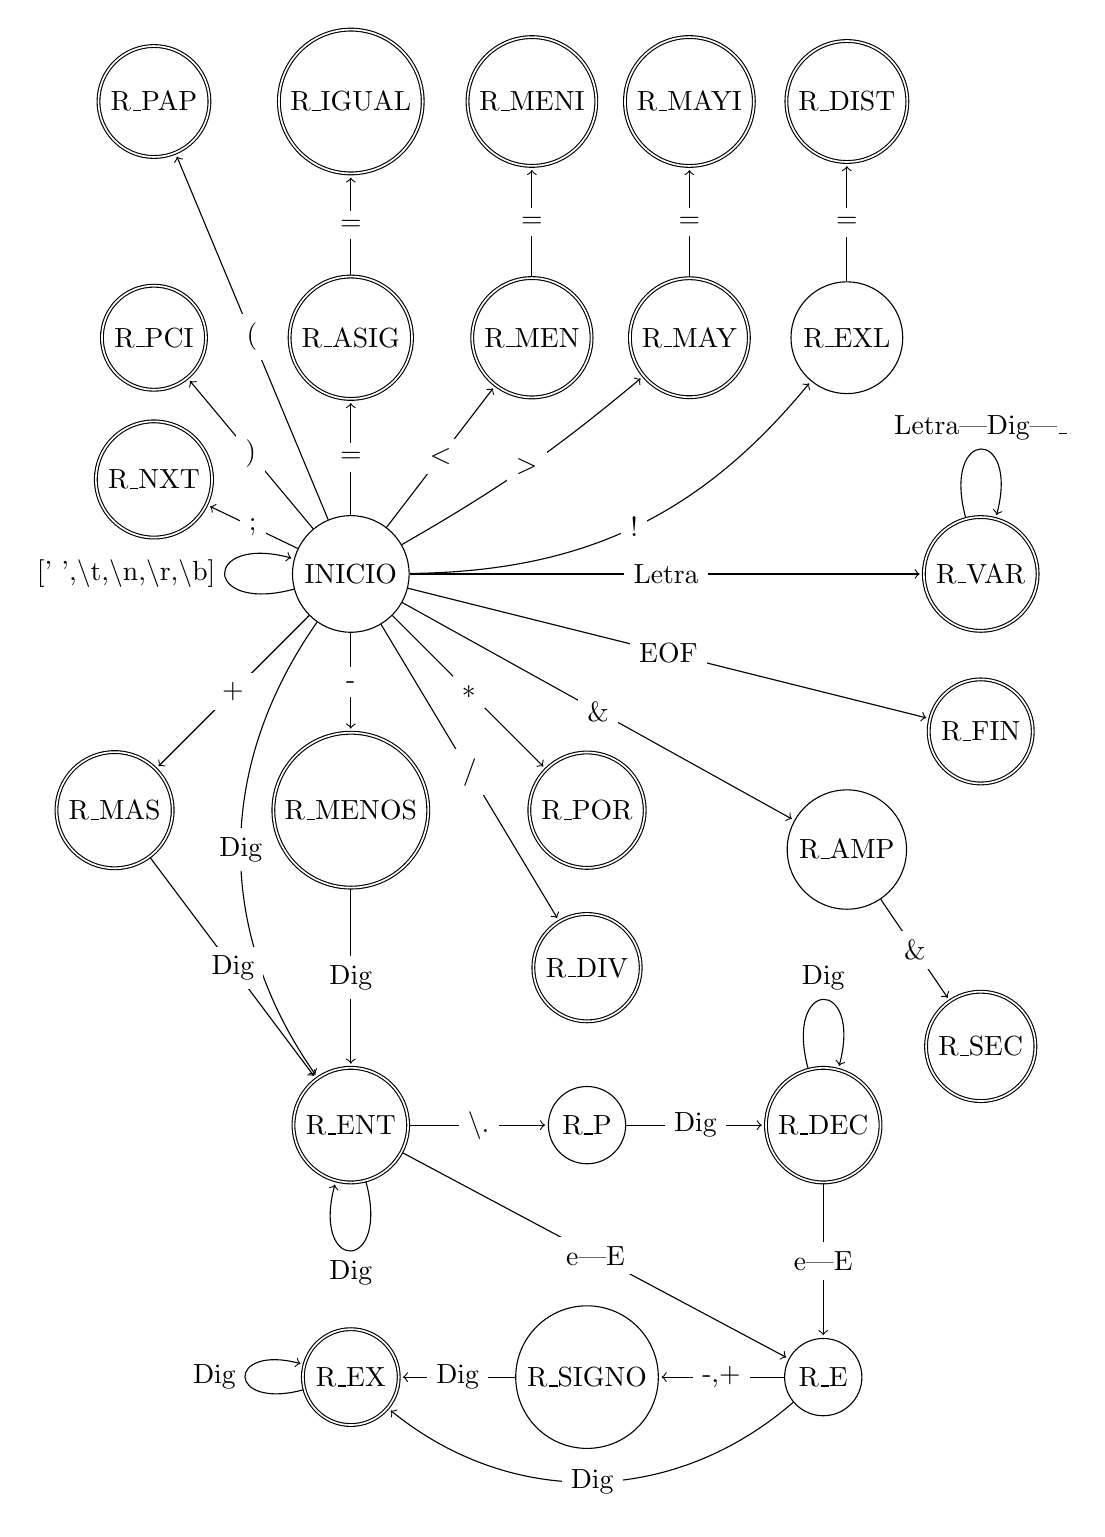
\begin{tikzpicture}[shorten >=1pt,node distance=2cm,on grid,auto]
    \node[state] (q_0) {INICIO};
    \node[state, accepting] (q_1) [above=3of q_0]  {R\_ASIG};
    \node[state, accepting] (q_2) [left=2.5of q_1] {R\_PCI};
    \node[state, accepting] (q_3) [above=3of q_2] {R\_PAP};
    \node[state, accepting] (q_4) [above=3of q_1] {R\_IGUAL};
    \node[state, accepting] (q_5) [right=2.3of q_1] {R\_MEN};
    \node[state, accepting] (q_6) [right=2of q_5] {R\_MAY};
    \node[state] (q_7) [right=2of q_6] {R\_EXL};
    \node[state, accepting] (q_8) [above=3of q_5] {R\_MENI};
    \node[state, accepting] (q_9) [above=3of q_6] {R\_MAYI};
    \node[state, accepting] (q_10) [above=3of q_7] {R\_DIST};
    \node[state, accepting] (q_11) [below=3of q_0] {R\_MENOS};
		\node[state, accepting] (q_12) [left=3of q_11] {R\_MAS};
    \node[state, accepting] (q_13) [right=3of q_11] {R\_POR};
    \node[state, accepting] (q_14) [below=of q_13] {R\_DIV};
    \node[state, accepting] (q_15) [below=4of q_11] {R\_ENT};
    \node[state] (q_16) [right=3of q_15] {R\_P};
    \node[state, accepting] (q_17) [right=3of q_16] {R\_DEC};
    \node[state] (q_18) [below=3.2of q_17] {R\_E};
    \node[state] (q_19) [left=3of q_18] {R\_SIGNO};
    \node[state, accepting] (q_20) [left=3of q_19] {R\_EX};
    \node[state, accepting] (q_21) [right=8of q_0] {R\_VAR};
    \node[state, accepting] (q_22) [below=2of q_21] {R\_FIN};
    \node[state] (q_23) [below=6.5of q_7] {R\_AMP};
    \node[state, accepting] (q_24) [below=4of q_22] {R\_SEC};
		\node[state, accepting] (q_25) [below=1.8of q_2] {R\_NXT};
			\path[->]
          (q_0) edge [loop left] node {$[$' ',\textbackslash t,\textbackslash n,\textbackslash r,\textbackslash b]} (q_0)
                edge node [fill=white, anchor=center, pos=0.5]          {=} (q_1)
                edge node [fill=white, anchor=center, pos=0.5]     {$)$} (q_2)
                edge node [fill=white, anchor=center, pos=0.5]           {$($} (q_3)
                edge node [fill=white, anchor=center, pos=0.5]           {$<$} (q_5)
                edge [bend right=5] node [fill=white, anchor=center, pos=0.5] {$>$} (q_6)
                edge [bend right=25] node [fill=white, anchor=center, pos=0.5] {!} (q_7)
                edge node [fill=white, anchor=center, pos=0.5] {-} (q_11)
                edge node [fill=white, anchor=center, pos=0.5] {+} (q_12)
                edge node [fill=white, anchor=center, pos=0.5] {$\ast$} (q_13)
                edge  node [fill=white, anchor=center, pos=0.5] {/} (q_14)
                edge [bend right=35]  node [fill=white, anchor=center, pos=0.5] {Dig} (q_15)
                edge  node [fill=white, anchor=center, pos=0.5] {Letra} (q_21)
                edge  node [fill=white, anchor=center, pos=0.5] {EOF} (q_22)
                edge  node [fill=white, anchor=center, pos=0.5] {\&} (q_23)
								edge  node [fill=white, anchor=center, pos=0.5] {;} (q_25)
          (q_1) edge  node[fill=white, anchor=center, pos=0.5]     {=} (q_4)
          (q_5) edge  node [fill=white, anchor=center, pos=0.5]            {=} (q_8)
          (q_6) edge  node [fill=white, anchor=center, pos=0.5]            {=} (q_9)
          (q_7) edge node [fill=white, anchor=center, pos=0.5] {=} (q_10)
          (q_11) edge node [fill=white, anchor=center, pos=0.5] {Dig} (q_15)
          (q_12) edge node [fill=white, anchor=center, pos=0.5] {Dig} (q_15)
          (q_15) edge [loop below] node {Dig} (q_15)
                 edge node [fill=white, anchor=center, pos=0.5] {\textbackslash .} (q_16)
                 edge node [fill=white, anchor=center, pos=0.5] {e|E} (q_18)
          (q_16) edge node [fill=white, anchor=center, pos=0.5] {Dig} (q_17)
          (q_17) edge [loop above] node {Dig} (q_17)
                 edge node [fill=white, anchor=center, pos=0.5] {e|E} (q_18)
          (q_18) edge [bend left=40] node [fill=white, anchor=center, pos=0.5] {Dig} (q_20)
                 edge node [fill=white, anchor=center, pos=0.5] {-,+} (q_19)
					(q_19) edge node [fill=white, anchor=center, pos=0.5] {Dig} (q_20)
					(q_20) edge [loop left] node {Dig} (q_20)
          (q_21) edge [loop above=0.5] node {Letra|Dig|\_} (q_21)
          (q_23) edge node [fill=white, anchor=center, pos=0.5] {\&} (q_24);
  \end{tikzpicture}
	
%---------------------------------------------------------------------
%                   Cap�tulo 2 - Analizador sint�ctico
%---------------------------------------------------------------------
\chapter{Fase 2: Analizador sint�ctico}
En esta fase desarrollaremos el analizador sint�ctico descendente predictivo para el lenguaje descrito en la primera fase. 
%---------------------------------------------------------------------
\section{Gram�tica incontextual}
%---------------------------------------------------------------------
\label{cap2:sec:gramatica_incontextual}

\subsection{Operadores}
Empezaremos definiendo la gram�tica incontextual que define el lenguaje. Los operadores que utiliza nuestro lenguaje aparecen en la tabla \ref{tabla:operadores}.

\begin{table}[htbp]
	\centering
		\begin{tabular}{|c|c|c|c|}
			\hline
			Operador & Prioridad & Tipo & Asociatividad \\
			\hline 
			+,- & 0 & Binario infijo & Asocia Izquierda \\ \hline
			\multirow{ 2}{*} and & {1} & {Binarios infijos} & Asocia Derecha \\ or & & & No asocia \\ \hline
			Relacionales & 2 & Binario infijo & No asocia \\ \hline
			*,/ & 3 & Binario infijo & Asocia Izquierda \\ \hline
			\multirow{ 2}{*} - & {4} & {Unarios prefijos} & Asocia \\ not & & & No asocia \\
			\hline
		\end{tabular}
		\caption{Operadores}
		\label{tabla:operadores}
\end{table}

\subsection{Gram�tica incontextual}
La gram�tica incotextual obtenida apartir de la definici�n y los operadores es la siguiente:

S $\rightarrow$ Programa \underline{EOF}

Programa $\rightarrow$ LDs \underline{SEC} LIs

LDs $\rightarrow$ LDs \underline{NXT} Declaracion

LDs $\rightarrow$ Declaracion

Declaracion $\rightarrow$ \underline{NUM} \underline{VAR}

Declaracion $\rightarrow$ \underline{BOOL} \underline{VAR}

LIs $\rightarrow$ LIs \underline{NXT} Instruccion

LIs $\rightarrow$ Instruccion

Instruccion $\rightarrow$ \underline{VAR} \underline{ASIG} EXP0

\

EXP0 $\rightarrow$ EXP0 OP0 EXP1

EXP0 $\rightarrow$ EXP1 

EXP1 $\rightarrow$ EXP2 \underline{AND} EXP1 

EXP1 $\rightarrow$ EXP2 \underline{OR} EXP2  

EXP1 $\rightarrow$ EXP2

EXP2 $\rightarrow$ EXP3 OP2 EXP3 

EXP2 $\rightarrow$ EXP3 

EXP3 $\rightarrow$ EXP3 OP3 EXP4 

EXP3 $\rightarrow$ EXP4 

EXP4 $\rightarrow$ \underline{MENOS} EXP4

EXP4 $\rightarrow$ \underline{NOT} EXP5 

EXP5 $\rightarrow$ \underline{NUMR}

EXP5 $\rightarrow$ \underline{VAR}

EXP5 $\rightarrow$ \underline{TRUE}

EXP5 $\rightarrow$ \underline{FALSE}

EXP5 $\rightarrow$ \underline{PAP} EXP0 \underline{PCIERRE} 

OP0 $\rightarrow$ \underline{MAS}

OP0 $\rightarrow$ \underline{MENOS} 

OP2 $\rightarrow$ \underline{MAY} 

OP2 $\rightarrow$ \underline{MEN} 

OP2 $\rightarrow$ \underline{MAYI} 

OP2 $\rightarrow$ \underline{MENI} 

OP2 $\rightarrow$ \underline{IGUAL} 

OP2 $\rightarrow$ \underline{DIST} 

OP3 $\rightarrow$ \underline{POR} 

OP3 $\rightarrow$ \underline{DIV} 

\subsection{Gram�tica transformada LL(1)}
Necesitamos transformar la gram�tica a una LL(1). Una vez transformada, la gram�tica queda de la siguiente manera:

S $\rightarrow$ Programa \underline{EOF}

Programa $\rightarrow$ LDs \underline{SEC} LIs

LDs $\rightarrow$ Declaracion RLDS

RLDS $\rightarrow$ \underline{NXT} Declaracion RLDS

RLDS $\rightarrow$ $\varepsilon$

Declaracion $\rightarrow$ \underline{NUM} \underline{VAR}

Declaracion $\rightarrow$ \underline{BOOL} \underline{VAR}

LIs $\rightarrow$ Instruccion RLIS

RLIS $\rightarrow$ \underline{NXT} Instruccion RLIS

RLIS $\rightarrow$ $\varepsilon$

Instruccion $\rightarrow$ \underline{VAR} \underline{ASIG} EXP0

\
	
EXP0 $\rightarrow$ EXP1 R0

R0 $\rightarrow$ OP0 EXP1 R0

R0 $\rightarrow$ $\varepsilon$

EXP1 $\rightarrow$ EXP2 R1

R1 $\rightarrow$ \underline{AND} EXP1

R1 $\rightarrow$ \underline{OR} EXP2  

R1 $\rightarrow$ $\varepsilon$

EXP2 $\rightarrow$ EXP3 R2 

R2 $\rightarrow$ OP2 EXP3 R2

R2 $\rightarrow$ $\varepsilon$ 

EX3 $\rightarrow$ EXP4 R3

R3 $\rightarrow$ OP3 EXP4 R3

R3 $\rightarrow$ $\varepsilon$

EXP4 $\rightarrow$ \underline{MENOS} EXP4

EXP4 $\rightarrow$ \underline{NOT} EXP5 

EXP4 $\rightarrow$ EXP5

EXP5 $\rightarrow$ \underline{NUMR}

EXP5 $\rightarrow$ \underline{VAR}

EXP5 $\rightarrow$ \underline{TRUE}

EXP5 $\rightarrow$ \underline{FALSE}

EXP5 $\rightarrow$ \underline{PAP} EXP0 \underline{PCIERRE} 

OP0 $\rightarrow$ \underline{MAS}

OP0 $\rightarrow$ \underline{MENOS} 

OP2 $\rightarrow$ \underline{MAY} 

OP2 $\rightarrow$ \underline{MEN} 

OP2 $\rightarrow$ \underline{MAYI} 

OP2 $\rightarrow$ \underline{MENI} 

OP2 $\rightarrow$ \underline{IGUAL} 

OP2 $\rightarrow$ \underline{DIST} 

OP3 $\rightarrow$ \underline{POR} 

OP3 $\rightarrow$ \underline{DIV} 

\subsection{Primeros y siguientes}
Los \textbf{primeros} de nuestra gram�tica son:

PRIM(S) = \{NUM, BOOL\}

PRIM(PROGRAMA) = \{NUM, BOOL\}

PRIM(LDS) = \{NUM, BOOL\}

PRIM(RLDS) = \{NXT\}

PRIM(DECLARACION) = \{NUM, BOOL\}

PRIM(LIS) = \{VAR\}

PRIM(RLIS) = \{NXT\}

PRIM(INSTRUCCION) = \{VAR\}

PRIM(R0) = \{MAS,MENOS\}

PRIM(R1) = \{AND,OR\}

PRIM(EXP1) = \{MENOS, NOT, NUMR, VAR, TRUE, FALSE, PAP\}

PRIM(EXP2) = \{MENOS, NOT, NUMR, VAR, TRUE, FALSE, PAP\}

PRIM(R2) = \{MAY, MEN, MAYI, MENI, IGUAL, DIST\}

PRIM(EXP3) = \{MENOS, NOT, NUMR, VAR, TRUE, FALSE, PAP\}

PRIM(R3) = \{POR, DIV, MENOS, NOT, NUMR, VAR, TRUE, FALSE, PAP\}

PRIM(EXP4) = \{MENOS, NOT, NUMR, VAR, TRUE, FALSE, PAP\}

PRIM(EXP5) = \{NUMR, VAR, TRUE, FALSE, PAP\}

PRIM(EXP0) = \{MENOS, NOT, NUMR, VAR, TRUE, FALSE, PAP\}

PRIM(OP0) = \{MAS, MENOS\}

PRIM(OP2) = \{MAY, MEN, MAYI, MENI, IGUAL, DIST\}

PRIM(OP3) = \{POR, DIV\}

Los \textbf{siguientes} son:

SIG(S) = \{$\varepsilon$\}

SIG(PROGRAMA) = \{EOF\}

SIG(LDS) = \{SEC\}

SIG(RLDS) = \{SEC\}

SIG(DECLARACION) = \{NXT, SEC\}

SIG(LIS) = \{EOF\}

SIG(RLIS) = \{EOF\}

SIG(INSTRUCCION) = \{NXT,EOF\}

SIG(R0) = \{PCI, NXT, EOF\}

SIG(R1) = \{PCI, MAS, MENOS, NXT, EOF\}

SIG(EXP1) = \{PCI, MAS, MENOS, NXT, EOF\}

SIG(EXP2) = \{PCI, AND, OR, MAS, MENOS, NXT, EOF\}

SIG(R2) = \{PCI, AND, OR, MAS, MENOS, NXT, EOF\}

SIG(EXP3) = \{PCI, MAY, MEN, MAYI, MENI, IGUAL, DIST, AND, OR, MAS, MENOS, NXT, EOF\}

SIG(R3) = \{PCI, MAY, MEN, MAYI, MENI, IGUAL, DIST, AND, OR, MAS, MENOS, NXT, EOF\}

SIG(EXP4) = \{PCI, POR, DIV, NOT, NUMR, VAR, TRUE, FALSE, PAP, MAY, MEN, MAYI, MENI, IGUAL, DIST, AND, OR, MAS, MENOS, NXT, EOF\}

SIG(EXP5) = \{PCI, POR, DIV, NOT, NUMR, VAR, TRUE, FALSE, PAP, MAY, MEN, MAYI, MENI, IGUAL, DIST, AND, OR, MAS, MENOS, NXT, EOF\}

SIG(EXP0) = \{PCI, NXT, EOF\}

SIG(OP0) = \{MENOS, NOT, NUMR, VAR, TRUE, FALSE, PAP\}

SIG(OP2) = \{MENOS, NOT, NUMR, VAR, TRUE, FALSE, PAP\}

SIG(OP3) = \{MENOS, NOT, NUMR, VAR, TRUE, FALSE, PAP\}

\subsection{Directores}
Obtenidos los primeros y los siguientes podemos proceder a calcular los \textbf{directores}:

DIR(S $\rightarrow$ Programa \underline{EOF}) = \{NUM, BOOL\}

DIR(Programa $\rightarrow$ LDs \underline{SEC} LIs \underline{EOF}) = \{NUM, BOOL\}

DIR(LDs $\rightarrow$ Declaracion RLDS) = \{NUM, BOOL\}

DIR(RLDS $\rightarrow$ \underline{NXT} Declaracion RLDS) = \{NXT\}

DIR(RLDS $\rightarrow$ $\varepsilon$) = \{SEC\}

DIR(Declaracion $\rightarrow$ \underline{NUM} \underline{VAR}) = \{NUM\}

DIR(Declaracion $\rightarrow$ \underline{BOOL} \underline{VAR}) = \{BOOL\}

DIR(LIs $\rightarrow$ Instruccion RLIS) = \{VAR\}

DIR(RLIS $\rightarrow$ \underline{NXT} Instruccion RLDS) = \{NXT\}

DIR(RLIS $\rightarrow$ $\varepsilon$) = \{EOF\}

DIR(Instruccion $\rightarrow$ \underline{VAR} \underline{ASIG} EXP0) = \{VAR\}
	
DIR(EXP0 $\rightarrow$ EXP1 R0) = \{MENOS, NOT, NUMR, VAR, TRUE, FALSE, PAP\}

DIR(R0 $\rightarrow$ OP0 EXP1 R0) = \{MAS, MENOS\}

DIR(R0 $\rightarrow$ $\varepsilon$) = \{PCI, NXT, EOF\}

DIR(EXP1 $\rightarrow$ EXP2 R1) = \{MENOS, NOT, NUMR, VAR, TRUE, FALSE, PAP\}

DIR(R1 $\rightarrow$ \underline{AND} EXP1 R1) = \{AND\} 

DIR(R1 $\rightarrow$ \underline{OR} EXP2) = \{OR\}  

DIR(R1 $\rightarrow$ $\varepsilon$) = \{PCI, MAS, MENOS, NXT, EOF\}

DIR(EXP2 $\rightarrow$ EXP3 R2) = \{MENOS, NOT, NUMR, VAR, TRUE, FALSE, PAP\}

DIR(R2 $\rightarrow$ OP2 EXP3 R2) = \{MAY, MEN, MAYI, MENI, IGUAL, DIST\} 

DIR(R2 $\rightarrow$ $\varepsilon$) = \{PCI, AND, OR, MAS, MENOS, NXT, EOF\} 

DIR(EX3 $\rightarrow$ EXP4 R3) = \{MENOS, NOT, NUMR, VAR, TRUE, FALSE, PAP\}

DIR(R3 $\rightarrow$ OP3 EXP4 R3) = \{MUL,DIV\}

DIR(R3 $\rightarrow$ $\varepsilon$) = \{PCI, MAY, MEN, MAYI, MENI, IGUAL, DIST, AND, OR, MAS, MENOS, NXT, EOF\}

DIR(EXP4 $\rightarrow$ \underline{MENOS} EXP4) = \{MENOS\}

DIR(EXP4 $\rightarrow$ \underline{NOT} EXP5) = \{NOT\} 

DIR(EXP4 $\rightarrow$ EXP5) = \{NUMR, VAR, TRUE, FALSE, PAP\}

DIR(EXP5 $\rightarrow$ \underline{NUMR}) = \{NUMR\}

DIR(EXP5 $\rightarrow$ \underline{VAR}) = \{VAR\}

DIR(EXP5 $\rightarrow$ \underline{TRUE}) = \{TRUE\}

DIR(EXP5 $\rightarrow$ \underline{FALSE}) = \{FALSE\}

DIR(EXP5 $\rightarrow$ \underline{PAP} EXP0 \underline {PCIERRE}) = \{PAP\} 

DIR(OP0 $\rightarrow$ \underline{MAS}) = \{MAS\}

DIR(OP0 $\rightarrow$ \underline{MENOS}) = \{MENOS\}

DIR(OP2 $\rightarrow$ \underline{MAY}) = \{MAY\} 

DIR(OP2 $\rightarrow$ \underline{MEN}) = \{MEN\} 

DIR(OP2 $\rightarrow$ \underline{MAYI}) = \{MAYI\} 

DIR(OP2 $\rightarrow$ \underline{MENI}) = \{MENI\}

DIR(OP2 $\rightarrow$ \underline{IGUAL}) = \{IGUAL\} 

DIR(OP2 $\rightarrow$ \underline{DIST}) = \{DIST\} 

DIR(OP3 $\rightarrow$ \underline{POR}) = \{POR\} 

DIR(OP3 $\rightarrow$ \underline{DIV}) = \{DIV\}

%---------------------------------------------------------------------
%                   Cap�tulo 3 - Analizador sint�ctico ascendente
%---------------------------------------------------------------------
\chapter{Fase 3: Analizador sint�ctico ascendente}
En esta fase desarrollaremos una versi�n diferente del analizador sint�ctico, esta vez ascendente LR. Se implementar� con JLex y Cup haciendo uso de la gram�tica incontextual desarrollada en la fase 2.

\end{document}



 
